\chapter{Opracowanie wyników}

Rozdział ten zawiera analizę wyników opisanego w~części~\ref{cha:implementacja}.


\section{Wielkość błędu}
asdasd

\section{Warianty opadu}

\section{Analiza wrażliwości na posterunki opadowe}
W~tej części przeprowadzono wpływ wyłączenia wskazanego posterunku opadowego (ograniczono się do wybory punktów zawartych w granicach wskazanej zlewni) na wynik działania omawianej metody. Pozwala to znaleźć odpowiedź na pytanie: \textit{Czy sieć istniejących posterunków opadowych jest wystarczająca?}, a~to pomoże podejmować decyzje o~zwiększaniu ilości owych posterunków bądź przeniesieniu w~inną lokalizację.

Rysunek~\ref{fig:identyfikatory} przedstawia identyfikatory wykluczanych z~analizy punktów, natomiast wiersze tabeli prezentują rezultat działania programu bez zadanego punktu.

\begin{figure}[!ht]
	\centering
	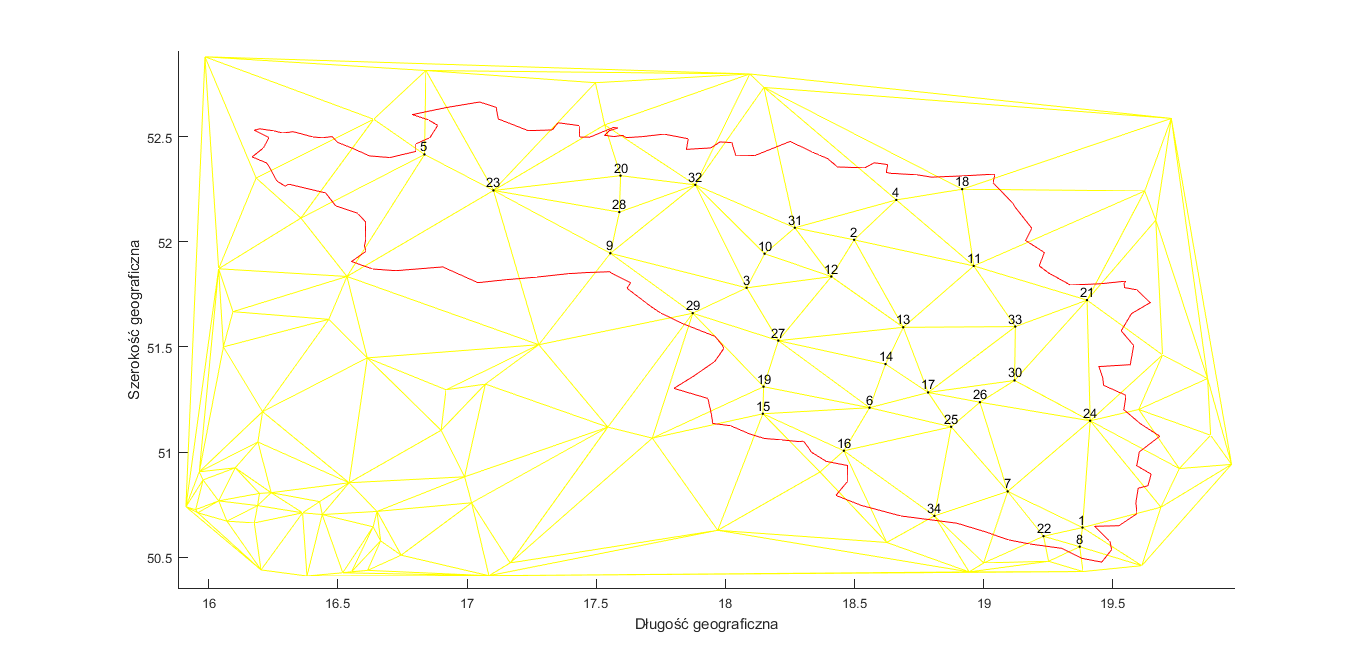
\includegraphics[width=1\linewidth]{identyfikatory_punktow}
	\label{fig:identyfikatory}
	\caption{Identyfikatory posterunków wewnątrz zlewni}
\end{figure}

\subsection{Opad paraboliczny}

\begin{table}
\label{tab:wyniki_wymierna}
\caption{Wpływ usunięcia posterunku na wynik algorytmu. Wariant paraboliczny.}
\begin{center}
\begin{tabular}{|c|l|l|r@{.}l|r@{.}l|r@{.}l|}
%nagłówek tabeli
\cline{2-3} \cline{6-9}
\multicolumn{1}{l}{} & \multicolumn{2}{|c|}{Opad $[m^3]$} & \multicolumn{2}{c}{} & \multicolumn{4}{|c|}{Wpływ posterunku} \\
\hline Posterunek & Wyznaczony & Rzeczywisty & \multicolumn{2}{c}{Różnica [\%]} & \multicolumn{2}{|c|}{[$m^3$]}& \multicolumn{2}{|c|}{$\times 10^{-3} [\%]$} \\ \hline \hline

0   &     1462995563.42529   &    1500568329.71548    &      2 & 5039  &             0 & 00          &     0 & 00 \\ \hline
1   &     1463076745.52465   &    1500568302.67758    &      2 & 4984  &         81182 & 099360466   &     5 & 55 \\ \hline
2   &     1461776787.89791   &    1500568329.71548    &      2 & 5851  &      -1218775 & 52738309    &   -83 & 31 \\ \hline
3   &     1462473733.66747   &    1500568329.71548    &      2 & 5386  &       -521829 & 757828236   &   -35 & 67 \\ \hline
4   &     1460378875.61033   &    1500568329.71547    &      2 & 6782  &      -2616687 & 81496501    &  -178 & 86 \\ \hline
5   &     1468988504.71699   &    1500568343.30161    &      2 & 1045  &       5992941 & 29169345    &   409 & 64 \\ \hline
6   &     1461622417.1231    &    1500568329.71548    &      2 & 5954  &      -1373146 & 30219698    &   -93 & 86 \\ \hline
7   &     1464682183.90386   &    1500568361.45334    &      2 & 3915  &       1686620 & 47856426    &   115 & 29 \\ \hline
%8   &     1462995563.42529   &    1500568329.71548    &      2 & 5039  &           -0 $ 00000405    &     0 & 00 \\ \hline
9   &     1453656531.65409   &    1500568329.71547    &      3 & 1262  &      -9339031 & 77120757    &  -638 & 35 \\ \hline
10  &     1462338580.82334   &    1500568329.71548    &      2 & 5476  &       -656982 & 601953506   &   -44 & 91 \\ \hline
11  &     1454316634.11975   &    1500568329.71548    &      3 & 0822  &      -8678929 & 30554771    &  -593 & 23 \\ \hline
12  &     1460880307.4094    &    1500568329.71548    &      2 & 6448  &      -2115256 & 01589155    &  -144 & 58 \\ \hline
13  &     1460206170.95541   &    1500568329.71548    &      2 & 6897  &      -2789392 & 46988297    &  -190 & 66 \\ \hline
14  &     1461450430.25043   &    1500568329.71547    &      2 & 6068  &      -1545133 & 17486525    &  -105 & 61 \\ \hline
15  &     1462002685.70473   &    1500568329.71548    &      2 & 5700  &       -992877 & 720560312   &   -67 & 87 \\ \hline
16  &     1462214551.12403   &    1500568329.71548    &      2 & 5559  &       -781012 & 301267624   &   -53 & 38 \\ \hline
17  &     1462691315.16175   &    1500568329.71548    &      2 & 5241  &       -304248 & 263546467   &   -20 & 80 \\ \hline
18  &     1464582760.98511   &    1500568329.71548    &      2 & 3981  &       1587197 & 55981994    &   108 & 49 \\ \hline
19  &     1461064560.9566    &    1500568329.71547    &      2 & 6325  &      -1931002 & 46868896    &  -131 & 99 \\ \hline
20  &     1461310691.73423   &    1500568329.71547    &      2 & 6161  &      -1684871 & 69106054    &  -115 & 17 \\ \hline
%21          1459561769.38071          1500568329.71548          2.73273529253659         -3433794.04457951       0.234709805718071
%22          1463418751.62474            1500568331.696          2.47570065864761          423188.199446678       -0.0289261437304617
%23          1453767799.36506          1500568329.71547           3.1188536652168         -9227764.06023598         0.630744500593777
%24          1462113590.39904          1500568331.17925          2.56267841864883           -881973.0262537        0.0602854204279846
%25          1461120846.70184          1500568329.71548          2.62883617043392         -1874716.72345448         0.128142338249148
%26          1462704787.16475          1500568329.71548          2.52328013332836         -290776.260545969        0.0198754027568736
%27          1460220263.75282          1500568329.71548          2.68885229440452         -2775299.67247844         0.189699801001492
%28          1461578202.47148          1500568329.71548          2.59835733381042         -1417360.95381665        0.0968807417637141
%29           1461321743.5352          1500568329.71548          2.61544812076069         -1673819.89008927         0.114410455638729
%30            1460813336.266          1500568329.71547          2.64932910166207         -2182227.15929556         0.149161570537257
%31          1460877238.93555          1500568329.71548          2.64507053720454         -2118324.48974419         0.144793637294742
%32          1461214840.52951          1500568329.71548            2.622572288556         -1780722.89578319         0.121717586867728
%33          1460597607.61728          1500568329.71547          2.66370556452917         -2397955.80801439         0.163907250846345
%34          1462056933.32981          1500568329.71548          2.56645403098514         -938630.095484972        0.0641580958241164



\end{tabular}
\end{center}
\end{table}


\subsection{Opad wymierny}

